\setchapterpreamble[u]{\margintoc}
\chapter{Intégration}
\labch{integration}

\todoinline{
Remarques générales :
}

% \todoinline{Il faudrait je pense mettre les illustrations dans un sous-dossier integration/ pour qu'on s'y retrouve à terme}

% \todoarmand{Les trois dernières animations du chapitre "Intégration sur un intervalle quelconque" sur votre site ne sont pas accessibles, est-ce normal ?}

% \todoinline{Une erreur dans un nom de dossier. J'ai corrigé. Si tu veux les sources python, je peux te les envoyer. C'est un peu à la main et je crois qu'il y a un outil plus performant maintenant...}


% \todoarmand{
% Inclure le flow chart \url{https://acamanes.github.io/psi/psi_doc/fc03.pdf} ? \\
% J'ai vu sur votre site que vous aviez fait plein de diagrammes pour les ECT. On pourrait inclure ceux sur l'intégration ?
% }

\todoinline{Flowcharts ajoutés. Je te laisse juger si ça vaut le coup de les mettre, je ne suis pas neutre sur ce sujet !}

\todoinline{Schéma à vérifier à la fin}

\begin{figure}[H]
    \centering
    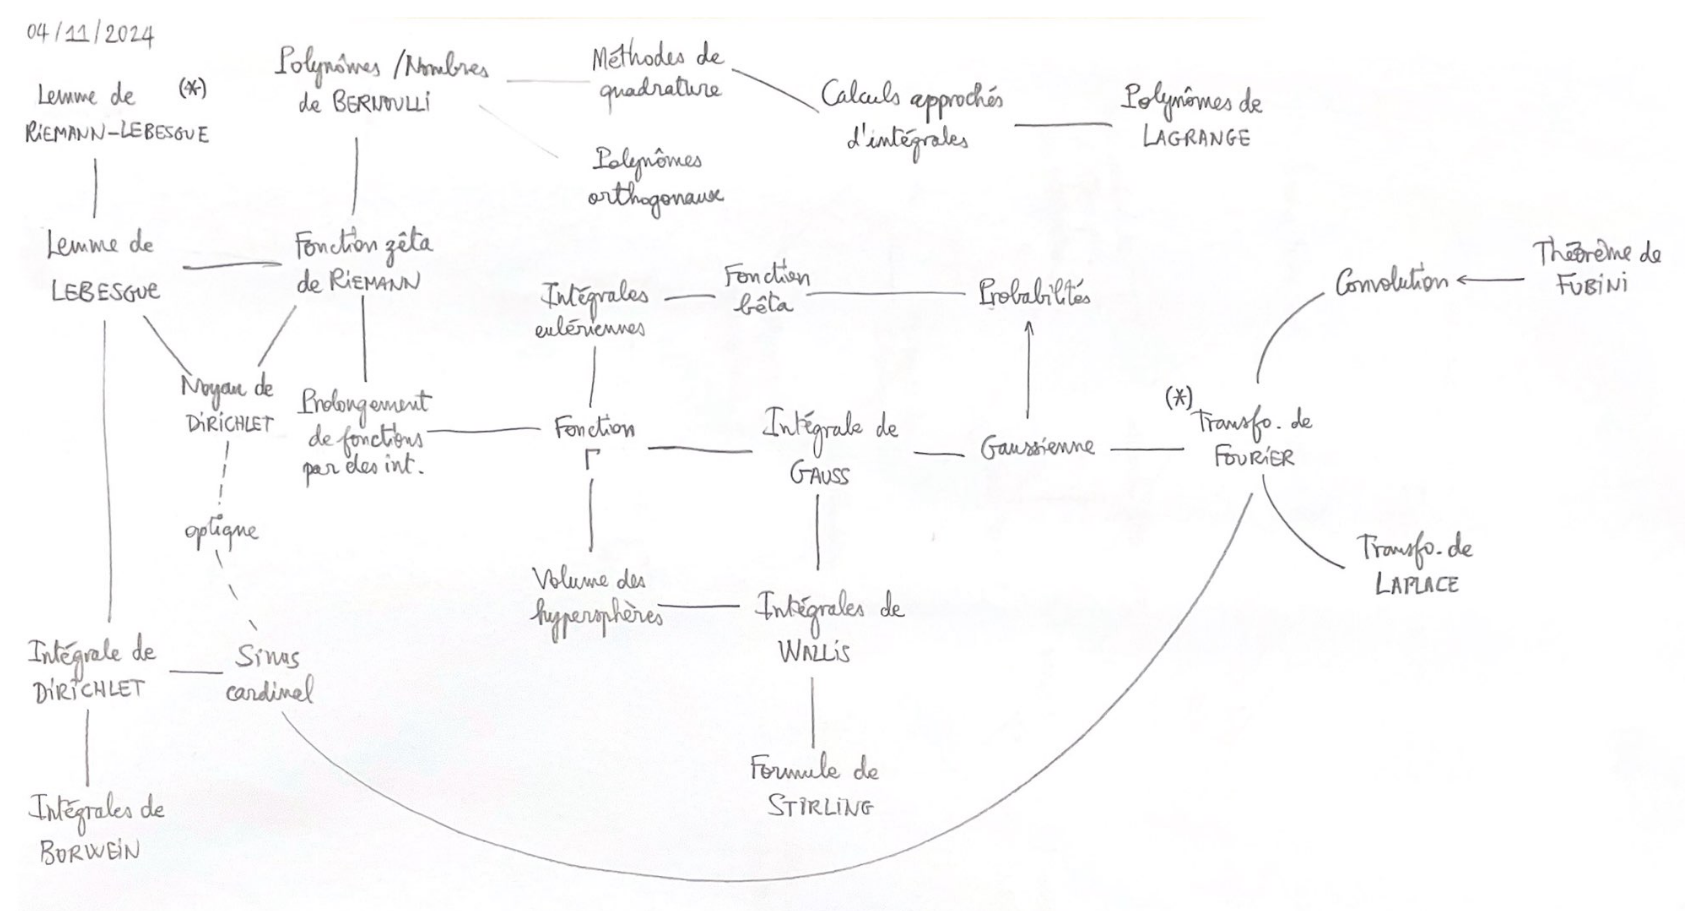
\includegraphics[width=1\linewidth]{chapitres/integration/documents/diagramme_integration.png}
    \caption{Ébauche d'un diagramme des chapitres}
\end{figure}

\todoinline{Chapitres validés (modulo la mise en page) : \\
01 : Alain : Validé\\
02 : Alain : Validé\\
03 : Alain : Validé (relire Simpson)\\
04 : Peut être un dessin de plus\\
05 : validé \\
07 : Ajouter un graphique ?.\\
08 : Supprimé et déplacé dans le 07\\
09 : TF gaussienne : supprimé car intégré au 10\\
09 : Produit de convolution ajouté\\
10 : Alain : Validé\\
11 : Quelques illustrations à terminer\\
12 : Presque validé. Illustrer les boules ?\\
13 : Presque validé après grosse modification pour bêta.\\
14 : Presque validé en supprimant le produit de convolution.\\
15 : Presque validé.\\
16 : Manque une illustration.\\
17 : déplacé en suites numériques.\\
18 : Illustrations à terminer.\\
19 : Validé - Illustrations à revoir\\
20 : Validé - Peut être à déplacer\\
21 : Validé - Manque peut être une illustration, mais ça ne me semble pas évident !\\
22 : Validé - Chercher une référence.
}

